\documentclass[a3paper,12pt]{extarticle} % Use extarticle for A3 paper size
\usepackage{graphicx} % Include this package for \includegraphics
\usepackage{amsmath}
\usepackage{amssymb} % Include this package for \mathbb
\usepackage[margin=1in]{geometry} % Adjust the margin as needed

\begin{document}

\author{kipngeno koech - bkoech}
\title{Homework 2 - Introduction to Probabilistic Graphical Models}   
\maketitle

\medskip

\maketitle
\section{Conditional Independence}
\begin{enumerate}
    \item (10 points) State True or False, and briefly justify your answer within 3 lines. The statements are either
    direct consequences of theorems in Koller and Friedman (2009, Ch. 3), or have a short proof. In the
    follows, P is a distribution and G is a BN structure.
    \begin{figure}[h!]
        \centering
        \includegraphics[width=0.5\textwidth]{"conditional_independence.png"}
        \caption{Caption for the image}
        \label{fig:example_image}
    \end{figure}
    \item Recall the definitions of local and global independences of G and independences of P.
    \begin{align}
        I_l(G) &= \{(X \perp \text{NonDescendants}_G(X) \mid \text{Parents}_G(X))\} \\
        I(G) &= \{(X \perp Y \mid Z) : \text{d-separated}_G(X, Y \mid Z)\} \\
        I(P) &= \{(X \perp Y \mid Z) : P(X, Y \mid Z) = P(X \mid Z)P(Y \mid Z)\}
    \end{align}
    \begin{enumerate}
        \item[(a)] In Figure \ref{fig:example_image}, relation 1 is true.
        \item[(b)] In Figure \ref{fig:example_image}, relation 2 is true.
        \item[(c)] In Figure \ref{fig:example_image}, relation 3 is true.
        \item[(d)] If G is an I-map for P, then P may have extra conditional independencies than G.
        \item[(e)] Two BN structures $G_1$ and $G_2$ are I-equivalent if they have the same skeleton and the same set of v-structures.
        \item[(f)] If $G_1$ is an I-map of distribution P, and $G_1$ has fewer edges than $G_2$, then $G_2$ is not a minimal I-map of P.
        \item[(g)] The P-map of a distribution, if it exists, is unique.
    \end{enumerate}
\end{enumerate}
\section{Exact Inference (Junction Tree a.k.a Clique Tree)}
\begin{enumerate}
    \item Consider the following Bayesian network G:
    \begin{figure}[h!]
        \centering
        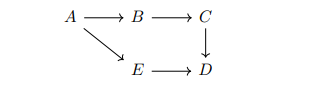
\includegraphics[width=0.5\textwidth]{junction_tree.png}
        \caption{Caption for the image}
        \label{fig:example_image}
    \end{figure}
    \item We are going to construct a junction tree T from G. Please sketch the generated objects in each step.
    \begin{enumerate}
        \item (4 points) Moralize G to construct an undirected graph H.
        \item (7 points) Triangulate H to construct a chordal graph H*.
        (Although there are many ways to triangulate a graph, for the ease of grading, please try adding fewest
        additional edges possible.)
        \item (7 points) Construct a cluster graph U where each node is a maximal clique Ci from H* and each edge is the sepset \(S_{i,j} = C_i \cap C_j\) between adjacent cliques \(C_i\) and \(C_j\).
        \item (7 points) The junction tree T is the maximum spanning tree of U.
        (The cluster graph is small enough to calculate maximum spanning tree in one’s head.)
    \end{enumerate}
\end{enumerate}

\end{document}